% Receiver schematic (Figure 2). R1: added for Referee 2, comment 2. R2: reference-sensor f0 label (Referee 1) and current receiver chain.
% Build: pdflatex receiver_schematic.tex  -> copy PDF to ../figures/receiver_schematic.pdf
\documentclass[border=2pt]{standalone}
\usepackage[T1]{fontenc}
\usepackage{lmodern}
\usepackage{amsmath}
\usepackage{tikz}
\usetikzlibrary{arrows.meta,positioning,calc,patterns,decorations.pathmorphing}
\begin{document}
\sffamily\footnotesize
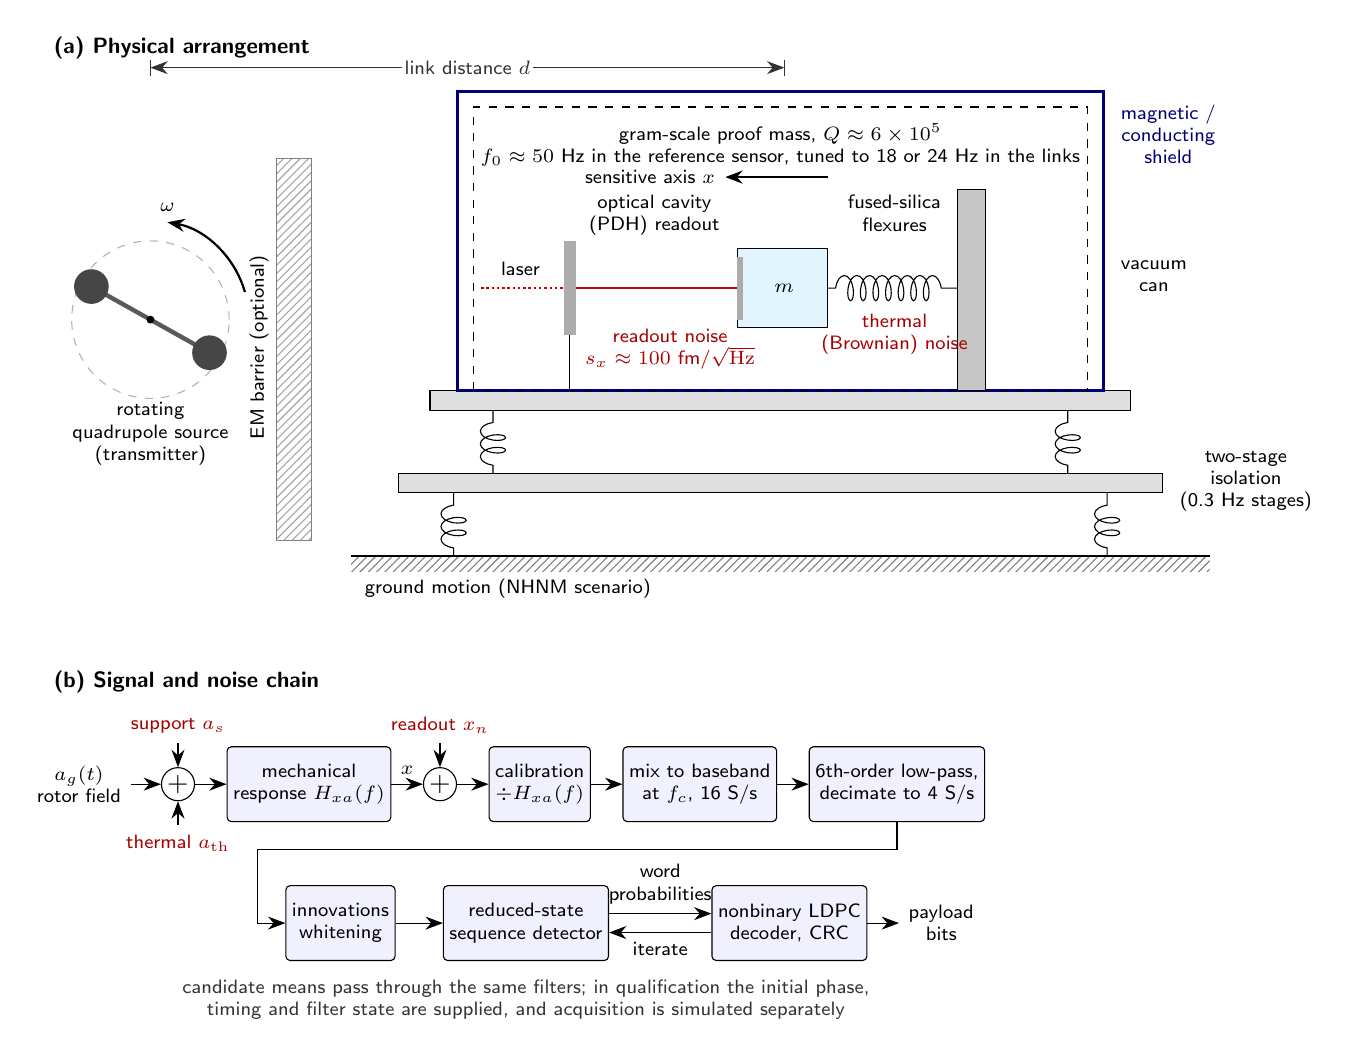
\begin{tikzpicture}[
  >={Stealth[length=2.2mm]},
  spring/.style={decorate,decoration={coil,aspect=0.45,segment length=1.6mm,amplitude=1.6mm,pre length=1mm,post length=1mm}},
  blk/.style={draw,rounded corners=1.5pt,fill=blue!6,align=center,minimum height=9.5mm,inner sep=2.2pt,font=\scriptsize\sffamily},
  sum/.style={draw,circle,inner sep=0pt,minimum size=4.2mm,fill=white},
  noise/.style={font=\scriptsize\sffamily,text=red!65!black,align=center},
  lab/.style={font=\scriptsize\sffamily,align=center}]

% ------------------------------------------------------------------ (a)
\node[anchor=west,font=\footnotesize\sffamily\bfseries] at (-0.2,7.0) {(a) Physical arrangement};

% rotor (top view)
\coordinate (rc) at (1.15,3.55);
\draw[gray!60,dashed] (rc) circle (1.0);
\draw[line width=1.6pt,gray!70!black] ($(rc)+(-0.75,0.42)$) -- ($(rc)+(0.75,-0.42)$);
\fill[gray!55!black] ($(rc)+(-0.75,0.42)$) circle (0.22) ($(rc)+(0.75,-0.42)$) circle (0.22);
\fill (rc) circle (0.05);
\draw[->,thick] ($(rc)+(1.2,0.35)$) arc[start angle=16,end angle=80,radius=1.25] node[above,lab] {$\omega$};
\node[lab] at (1.15,2.1) {rotating\\ quadrupole source\\ (transmitter)};

% barrier
\fill[pattern=north east lines,pattern color=gray!70] (2.75,0.75) rectangle (3.2,5.6);
\draw[gray] (2.75,0.75) rectangle (3.2,5.6);
\node[lab,rotate=90] at (2.53,3.2) {EM barrier (optional)};

% ground and isolation
\fill[pattern=north east lines,pattern color=gray] (3.7,0.35) rectangle (14.6,0.55);
\draw[thick] (3.7,0.55) -- (14.6,0.55);
\node[lab,anchor=west] at (3.75,0.13) {ground motion (NHNM scenario)};
\draw[spring] (5.0,0.55) -- (5.0,1.35);  \draw[spring] (13.3,0.55) -- (13.3,1.35);
\fill[gray!25] (4.3,1.35) rectangle (14.0,1.6); \draw (4.3,1.35) rectangle (14.0,1.6);
\draw[spring] (5.5,1.6) -- (5.5,2.4);    \draw[spring] (12.8,1.6) -- (12.8,2.4);
\fill[gray!25] (4.7,2.4) rectangle (13.6,2.65); \draw (4.7,2.4) rectangle (13.6,2.65);
\node[lab,anchor=west] at (14.1,1.5) {two-stage\\ isolation\\ (0.3 Hz stages)};

% vacuum can and shield
\draw[line width=1.1pt,blue!45!black] (5.05,2.65) rectangle (13.25,6.45);
\draw[dashed] (5.25,2.65) rectangle (13.05,6.25);
\node[lab,anchor=west,text=blue!45!black] at (13.35,5.9) {magnetic /\\ conducting\\ shield};
\node[lab,anchor=west] at (13.35,4.1) {vacuum\\ can};

% optical readout
\fill[gray!65] (6.4,3.35) rectangle (6.55,4.55);
\draw[red!80!black,line width=0.9pt] (6.55,3.95) -- (8.6,3.95);
\draw[red!80!black,line width=0.9pt,densely dotted] (5.35,3.95) -- (6.4,3.95);
\node[lab,anchor=south] at (7.55,4.5) {optical cavity\\ (PDH) readout};
\node[noise,anchor=north] at (7.75,3.55) {readout noise\\ $s_x\approx100$ fm/$\sqrt{\mathrm{Hz}}$};
\node[lab,anchor=south] at (5.85,3.98) {laser};

% proof mass, flexure, frame
\fill[cyan!12] (8.6,3.45) rectangle (9.75,4.45); \draw (8.6,3.45) rectangle (9.75,4.45);
\fill[gray!65] (8.6,3.55) rectangle (8.68,4.35);
\node[lab] at (9.2,3.95) {$m$};
\fill[gray!45] (11.4,2.65) rectangle (11.75,5.2); \draw (11.4,2.65) rectangle (11.75,5.2);
\draw (6.475,3.35) -- (6.475,2.65);
\draw[spring] (9.75,3.95) -- (11.4,3.95);
\node[lab,anchor=south] at (10.6,4.55) {fused-silica\\ flexures};
\node[noise,anchor=north] at (10.6,3.75) {thermal\\ (Brownian) noise};
\node[lab,anchor=north] at (9.15,6.17) {gram-scale proof mass, $Q\approx6\times10^5$\\ $f_0\approx50$ Hz in the reference sensor, tuned to 18 or 24 Hz in the links};
% sensitive axis and distance
\draw[->,thick] (9.75,5.36) -- (8.45,5.36) node[left,lab] {sensitive axis $x$};
\draw[<->,gray!40!black] (1.15,6.75) -- (9.2,6.75) node[midway,fill=white,lab,inner sep=1pt] {link distance $d$};
\draw[gray!40!black] (1.15,6.65) -- (1.15,6.85) (9.2,6.65) -- (9.2,6.85);

% ------------------------------------------------------------------ (b)
\begin{scope}[yshift=-0.6cm]
\node[anchor=west,font=\footnotesize\sffamily\bfseries] at (-0.2,-0.45) {(b) Signal and noise chain};
\node[lab,anchor=east] (in) at (0.9,-1.75) {$a_g(t)$\\ rotor field};
\node[sum] (s1) at (1.5,-1.75) {$+$};
\node[noise,above=3mm of s1] (sup) {support $a_s$};
\node[noise,below=3mm of s1] (th) {thermal $a_{\rm th}$};
\node[blk,right=4mm of s1] (mech) {mechanical\\ response $H_{xa}(f)$};
\node[sum,right=4mm of mech] (s2) {$+$};
\node[noise,above=3mm of s2] (ro) {readout $x_n$};
\node[blk,right=4mm of s2] (cal) {calibration\\ $\div H_{xa}(f)$};
\node[blk,right=4mm of cal] (mix) {mix to baseband\\ at $f_c$, 16 S/s};
\node[blk,right=4mm of mix] (lpf) {6th-order low-pass,\\ decimate to 4 S/s};
\draw[->] (in) -- (s1); \draw[->] (sup) -- (s1); \draw[->] (th) -- (s1);
\draw[->] (s1) -- (mech); \draw[->] (mech) -- node[above,lab] {$x$} (s2); \draw[->] (ro) -- (s2);
\draw[->] (s2) -- (cal); \draw[->] (cal) -- (mix); \draw[->] (mix) -- (lpf);

\node[blk,below=8mm of mech,xshift=4mm] (wh) {innovations\\ whitening};
\node[blk,right=6mm of wh] (det) {reduced-state\\ sequence detector};
\node[blk,right=13mm of det] (dec) {nonbinary LDPC\\ decoder, CRC};
\node[lab,right=4mm of dec] (out) {payload\\ bits};
\draw[->] (lpf.south) -- ++(0,-0.35) -| ($(wh.west)+(-0.35,0)$) -- (wh.west);
\draw[->] (wh) -- (det); \draw[->] ([yshift=1.2mm]det.east) -- node[above,lab] {word\\ probabilities} ([yshift=1.2mm]dec.west);
\draw[->] ([yshift=-1.2mm]dec.west) -- node[below,lab] {iterate} ([yshift=-1.2mm]det.east); \draw[->] (dec) -- (out);
\node[lab,anchor=north,text=gray!40!black,text width=12cm] at ($(det.south)+(0,-0.12)$)
  {candidate means pass through the same filters; in qualification the initial phase, timing and filter state are supplied, and acquisition is simulated separately};
\end{scope}
\end{tikzpicture}
\end{document}
